\begin{appendices}
\chapter{WBS}

\section{Previous WBS}
This is where the Work Breakdown Structures from early development is placed here with the most recent placed earliest, as can be seen in Figures \ref{fig:WBS222}, \ref{fig:WBS13}, \ref{fig:WBS83}, \ref{fig:WBS153}, \ref{fig:WBS223}, \ref{fig:WBS54}, and \ref{fig:WBSfin}.

\begin{figure}[p]
\setlength\fboxsep{0pt}
\setlength\fboxrule{1pt}\noindent\makebox[\textwidth]{%
 \fbox{
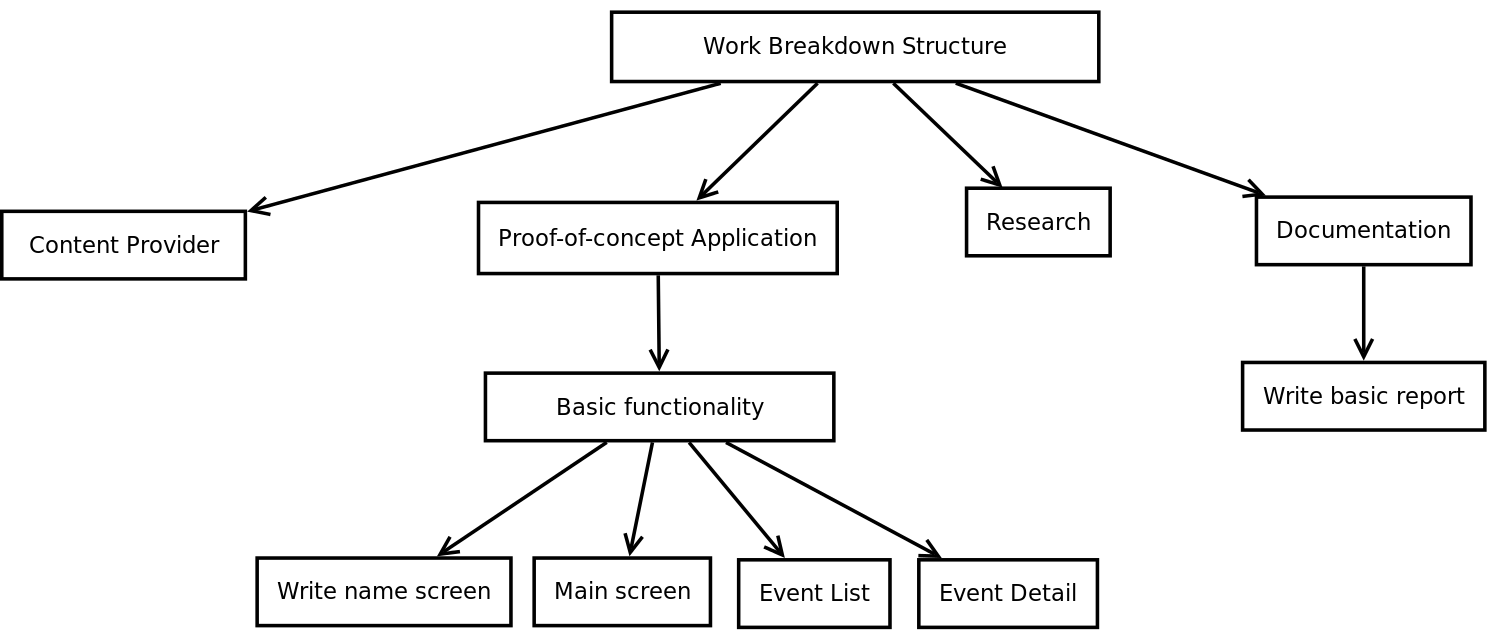
\includegraphics[width=1.45\textwidth , angle=270]{Res/WBSfirst.png}}}
\caption{The WBS as per 22.2.13 }
\label{fig:WBS222}
\end{figure}

\begin{figure}[p]
\setlength\fboxsep{0pt}
\setlength\fboxrule{1pt}\noindent\makebox[\textwidth]{%
 \fbox{
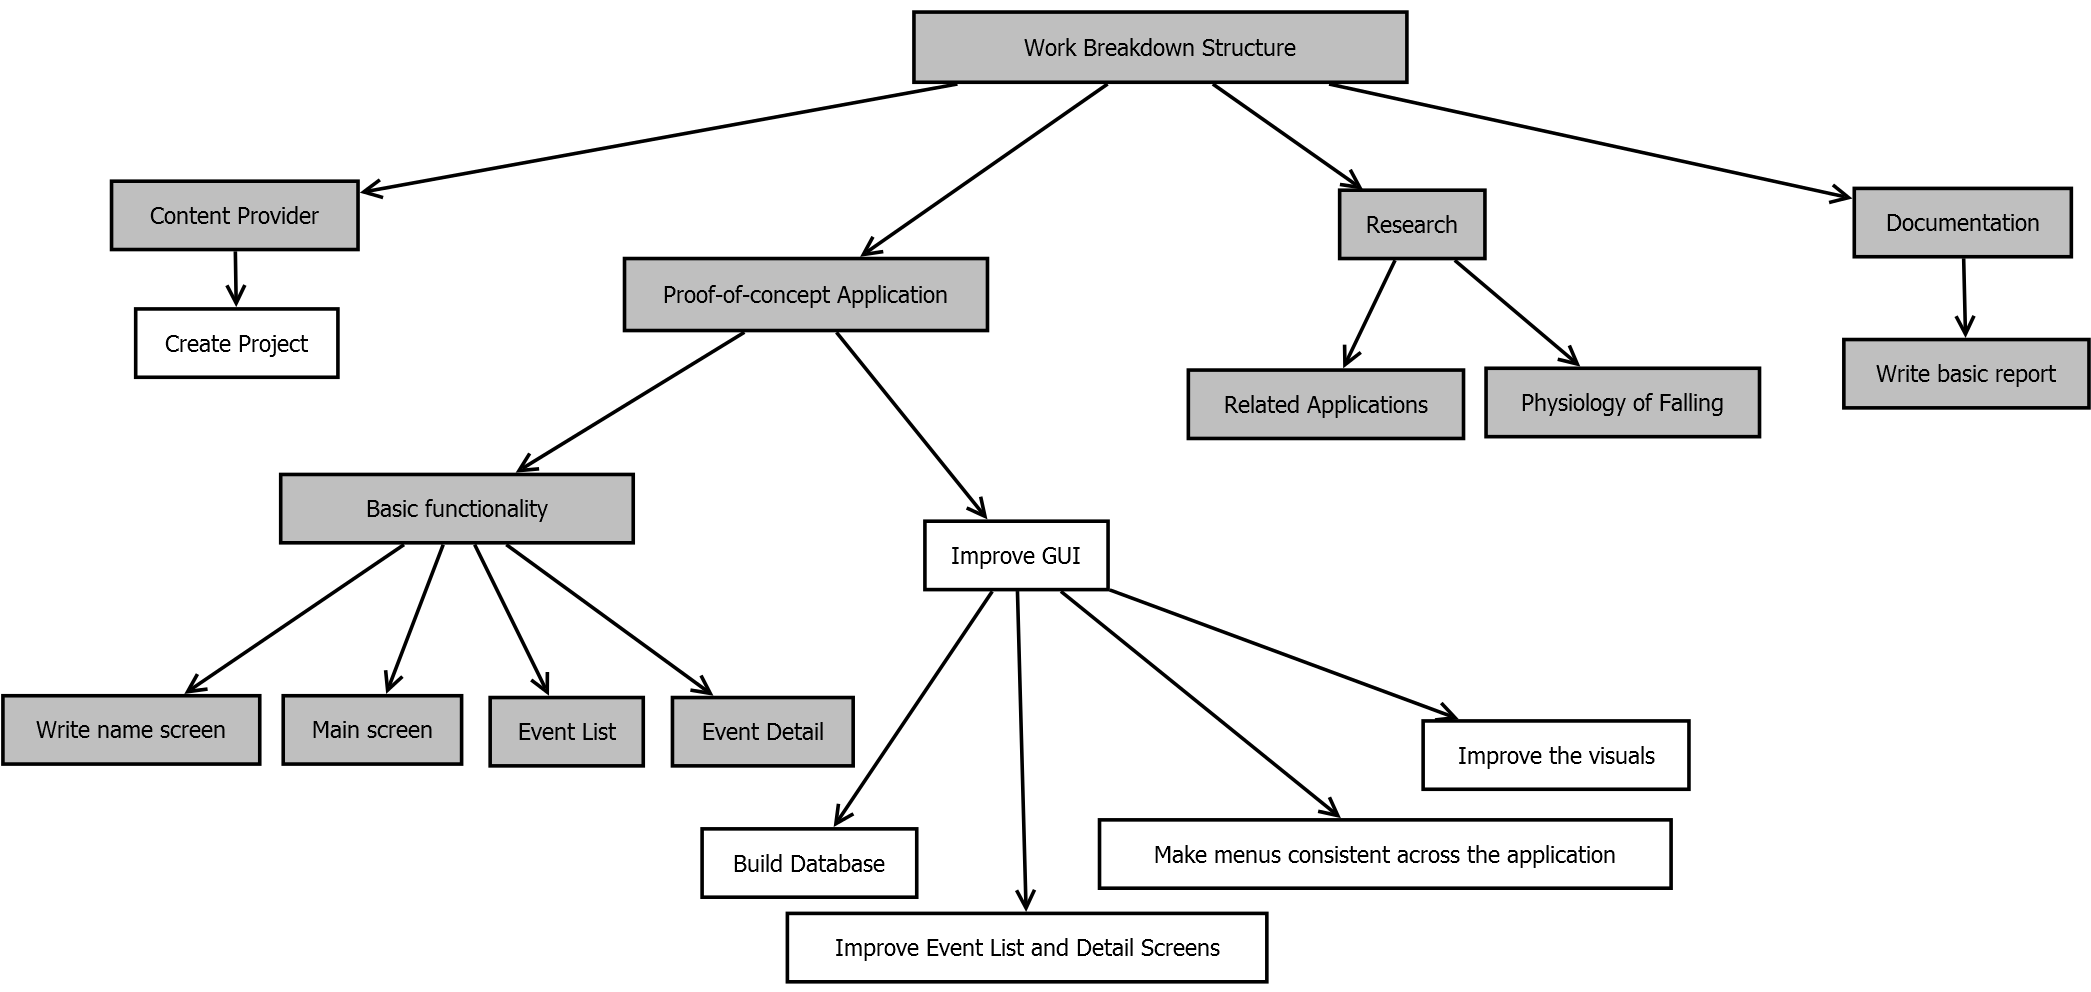
\includegraphics[width=1.45\textwidth , angle=270]{Res/WBS01313.png}}}
\caption{The WBS as per 1.3.13}
\label{fig:WBS13}
\end{figure}


\begin{figure}[p]
\setlength\fboxsep{0pt}
\setlength\fboxrule{1pt}\noindent\makebox[\textwidth]{%
 \fbox{
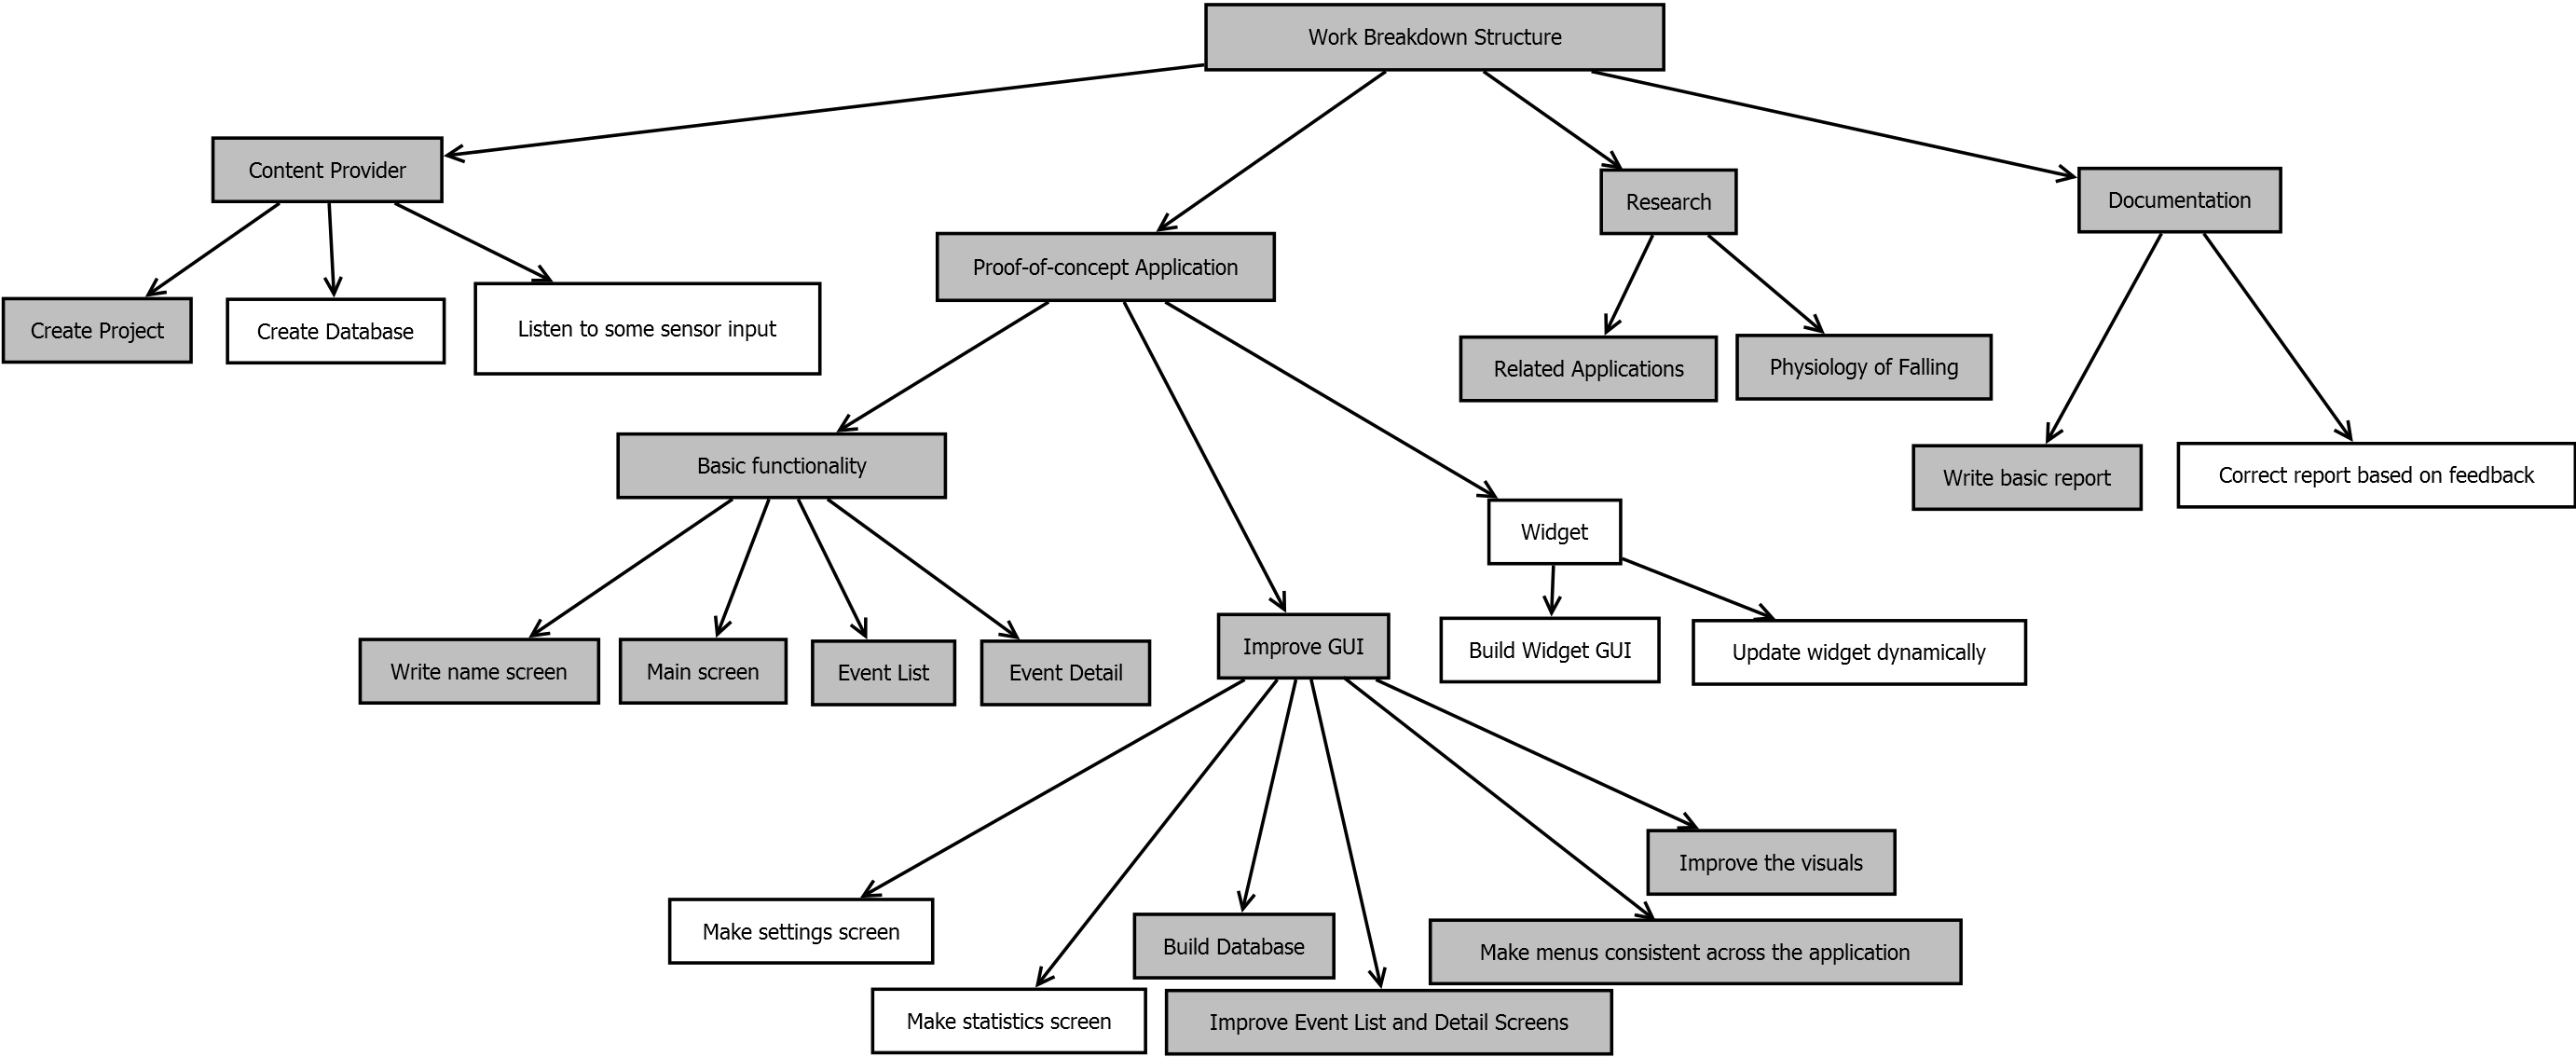
\includegraphics[width=1.45\textwidth , angle=270]{Res/WBS08313.png}}}
\caption{The WBS as per 8.3.13}
\label{fig:WBS83}
\end{figure}

\begin{figure}[p]
\setlength\fboxsep{0pt}
\setlength\fboxrule{1pt}\noindent\makebox[\textwidth]{%
 \fbox{
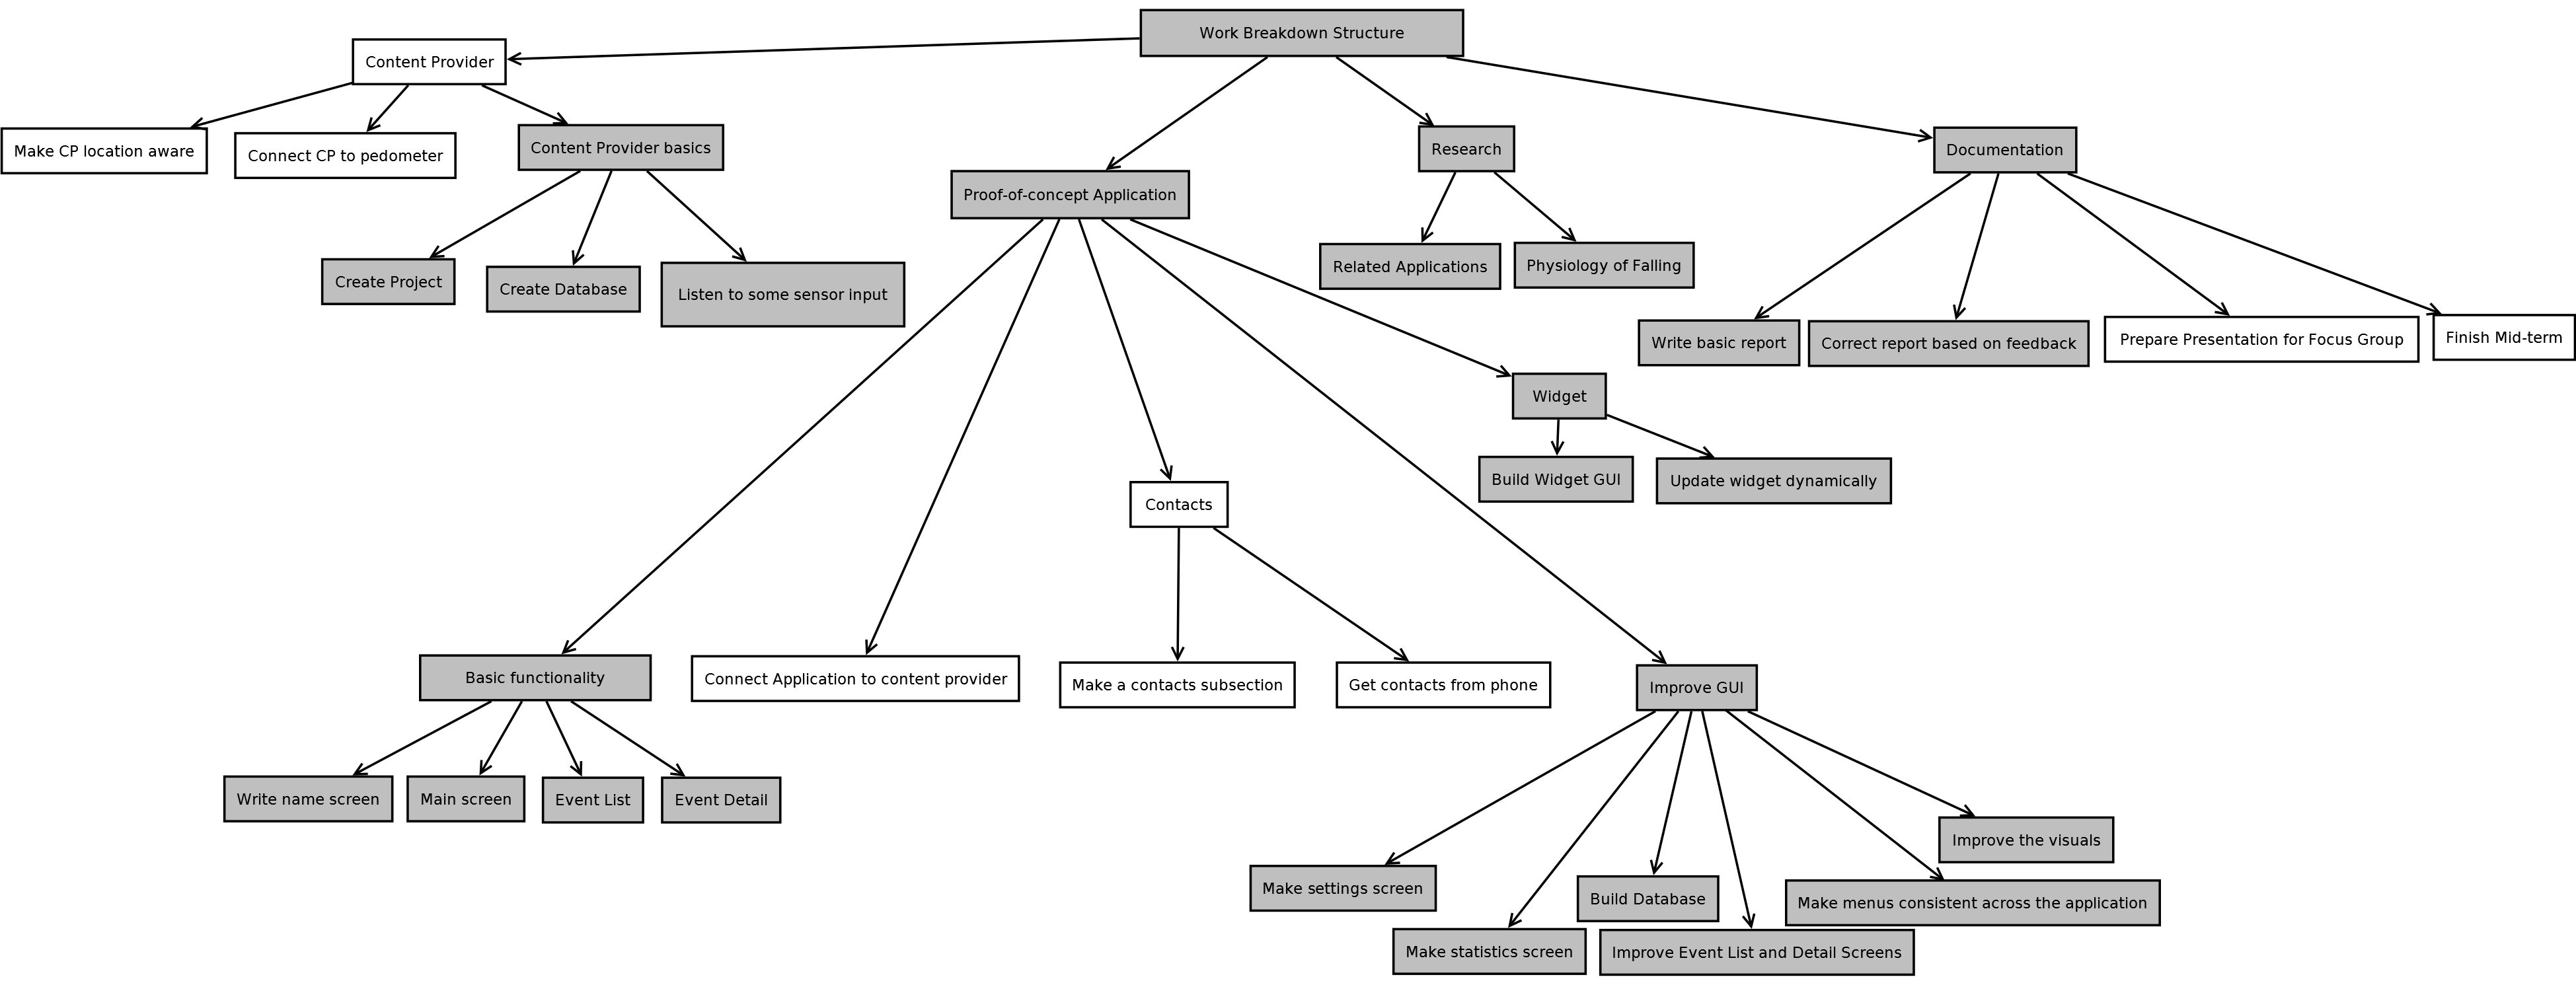
\includegraphics[width=1.45\textwidth , angle=270]{Res/WBS15313.png}}}
\caption{The WBS as per 15.3.13}
\label{fig:WBS153}
\end{figure}

\begin{figure}[p]
\setlength\fboxsep{0pt}
\setlength\fboxrule{1pt}\noindent\makebox[\textwidth]{%
 \fbox{
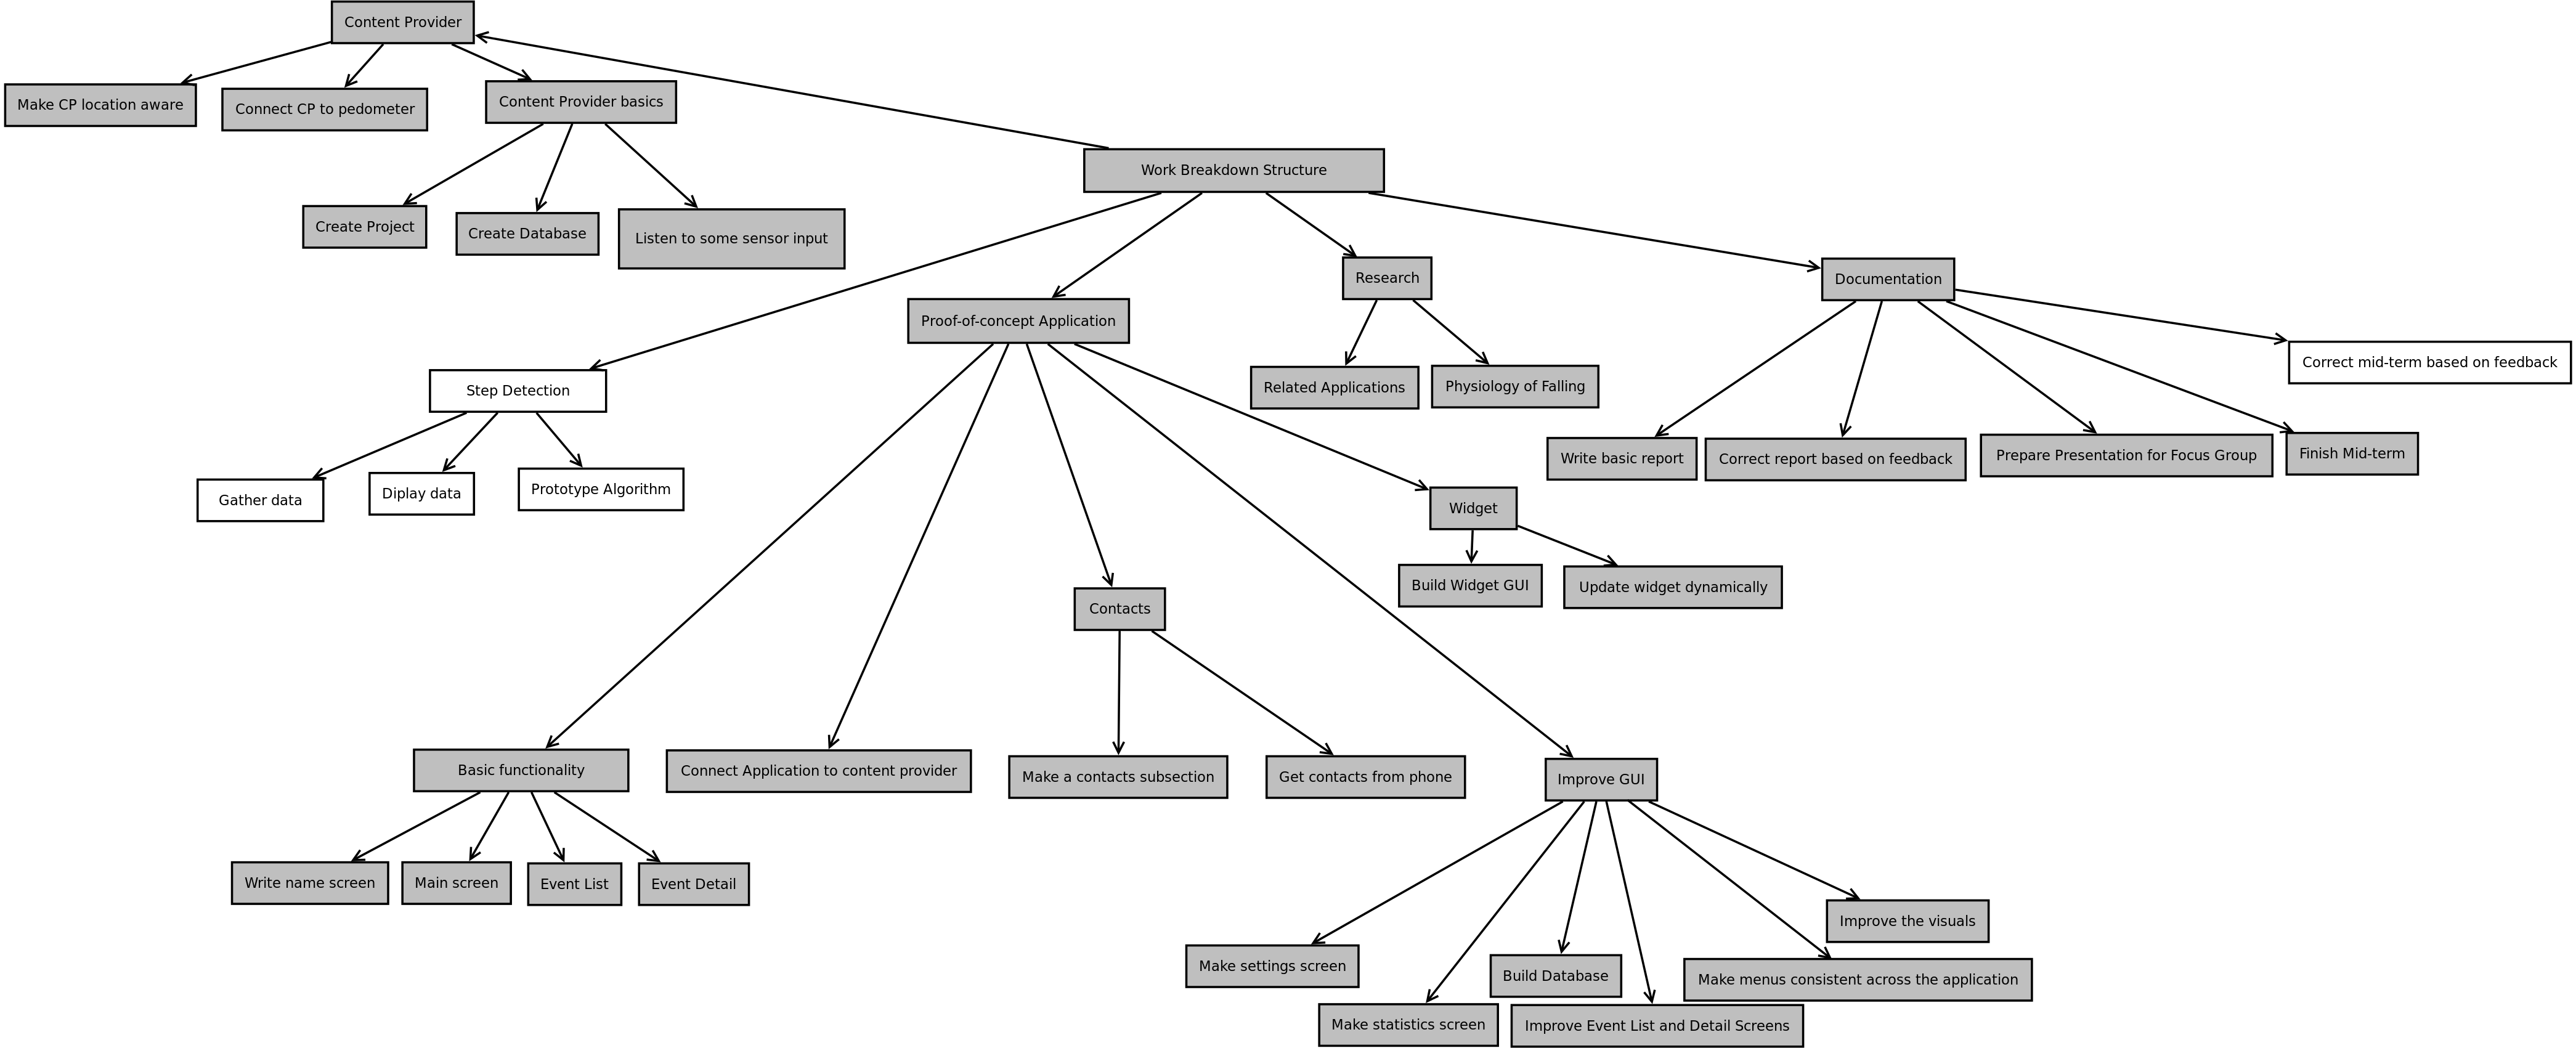
\includegraphics[width=1.45\textwidth , angle=270]{Res/WBS22313.png}}}
\caption{The WBS as per 22.3.13}
\label{fig:WBS223}
\end{figure}

\begin{figure}[p]
\setlength\fboxsep{0pt}
\setlength\fboxrule{1pt}\noindent\makebox[\textwidth]{%
 \fbox{
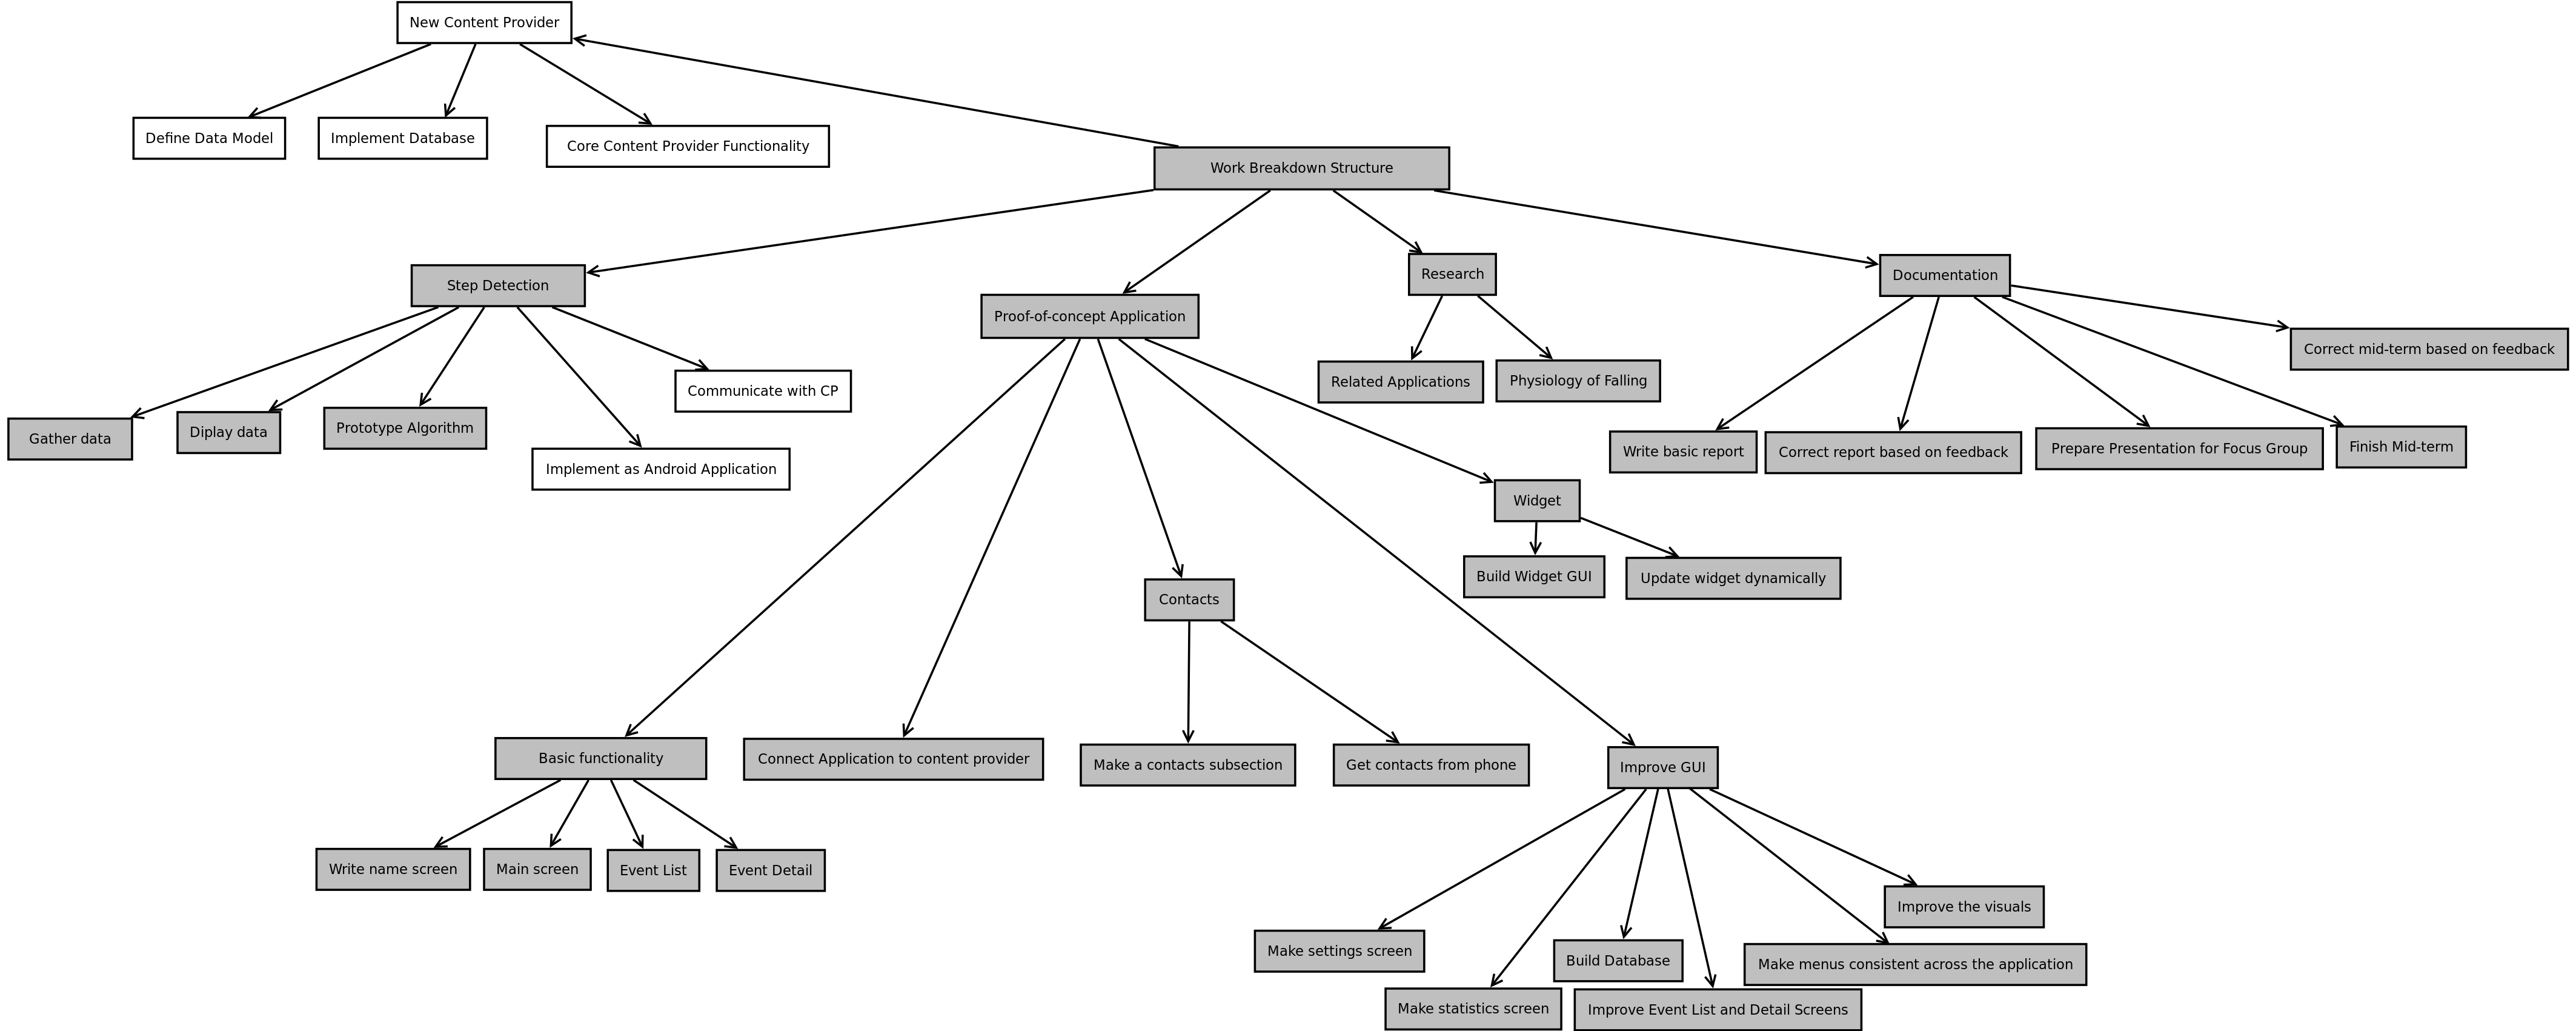
\includegraphics[width=1.45\textwidth , angle=270]{Res/WBS05413.png}}}
\caption{The WBS as per 5.4.13}
\label{fig:WBS54}
\end{figure}

\begin{figure}[p]
\setlength\fboxsep{0pt}
\setlength\fboxrule{1pt}\noindent\makebox[\textwidth]{%
 \fbox{
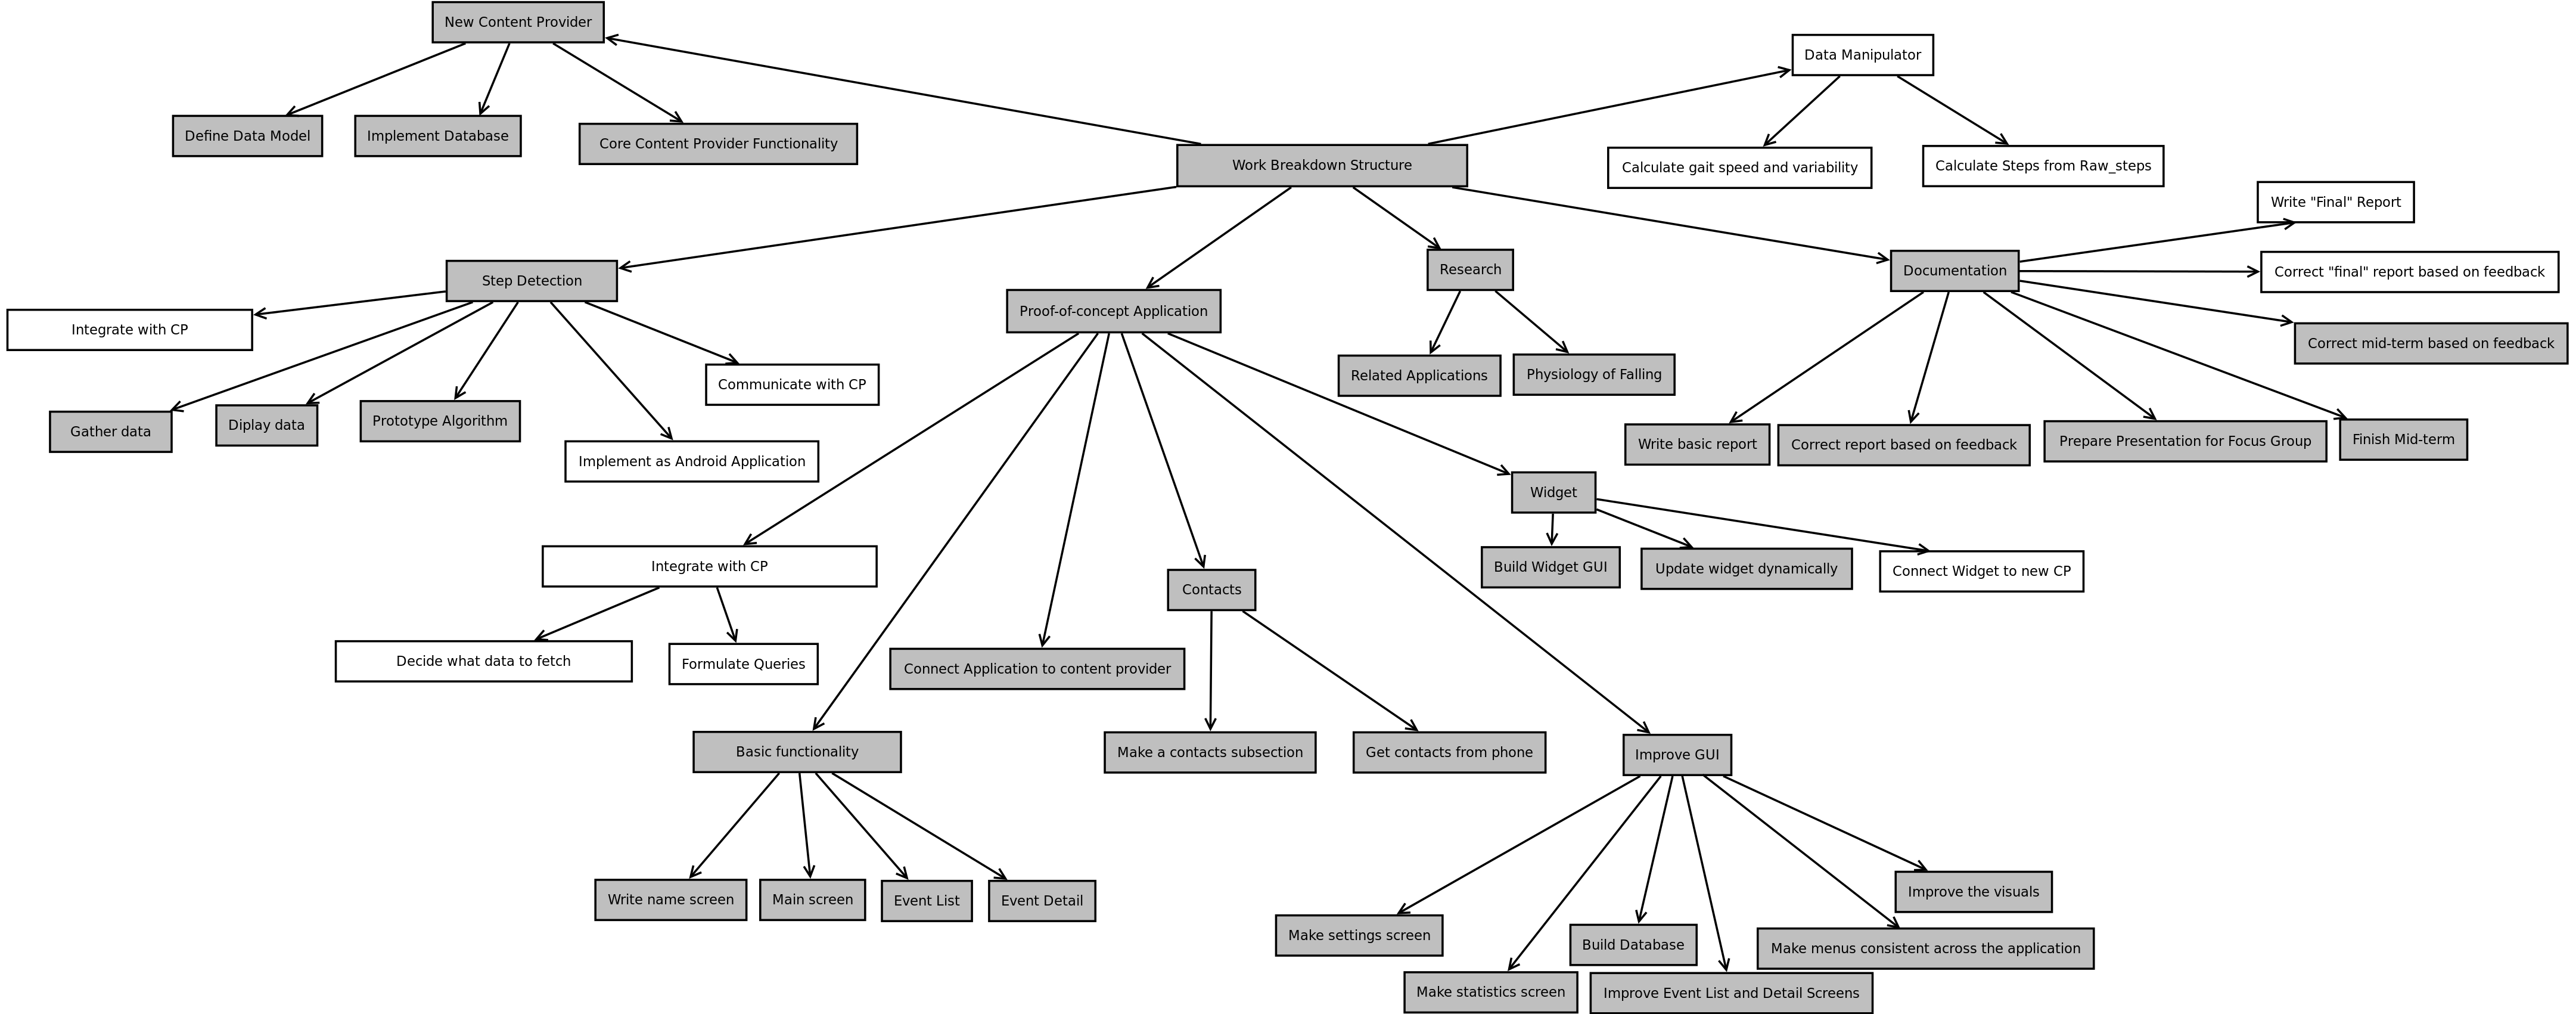
\includegraphics[width=1.45\textwidth , angle=270]{Res/WBSlast.png}}}
\caption{The final WBS}
\label{fig:WBSfin}
\end{figure}

%\section{Reports}

\chapter{Work summary}
\section{Sprint summaries}
\label{tab:sprintList}
The following is a list of the sprints:

\begin{description}
\item[Sprint 1: 01.02.13 - 08.02.13] \hline \hfill \\
User stories and paper prototypes of the GUI were developed.
\item[Sprint 2: 08.02.13 - 15.02.13] \hline \hfill \\
The group focused on learning Android development. New GUI paper prototypes were developed based on customer feedback. A mock-up application demonstrating core parts of the GUI was developed.
\item[Sprint 3: 15.02.13 - 22.02.13] \hline \hfill \\
Continued efforts on learning Android development. The mock-up was developed further. Research was conducted on the application domain, and on related applications. 
\item[Sprint 4: 22.02.13 - 01.03.13] \hline \hfill \\
The prototype application was expanded with a database, GUI visuals were improved, menu usage was made consistent throughout the prototype. The group tried to familiarize themselves with Content Providers in Android.
\item[Sprint 5: 01.03.13 - 08.03.13] \hline \hfill \\
A Content Provider was developed, incorporated the step detection from the Pedometer open-source application. Some secondary screens (settings and statistics) were implemented. Basic widget created.
\item[Sprint 6: 08.03.13 - 15.03.13] \hline \hfill \\
Widget was connected successfully to the main application. Application connected to the Content Provider. Work on report for the mid-term hand-in. Presentation for the focus group prepared. Unsuccessful attempts at making the Pedometer/Content Provider location aware. Implementation of contact management. 
\item[Sprint 7: 15.03.13 - 22.03.13] \hline \hfill \\
Research and development of step detection algorithm: Sensor data collection application developed, python scripts for displaying data and prototyping of algorithm. Work on Javadoc and code refactoring. Correction of report based on mid-term feedback.
\item[Ester holidays: 23.03.13 - 02.04.13] \hline \hfill \\
Little work was done due to the holidays.
\item[Sprint 9: 03.04.13 - 05.04.13] \hline \hfill \\
New system architecture was designed. Step detection algorithm implemented as Android application. The old Content Provider/Pedometer discarded, and new Content Provider implemented. 
\item[Sprint 10: 05.04.13 - 12.04.13] \hline \hfill \\
Efforts were focused on bug-fixing and integration of the three components. 
\item[Sprint 11: 13.04.13 - 19.04.13] \hline \hfill \\
Work on final report and small adjustments the integration of the components. The code underwent refactoring and commenting. 
\end{description}
\section{Meeting summaries}
Regular status reports was a part of necessary documentation. Of particular importance was reports to the supervisor, and reports done to the other group members. This status report was written during sprint 4. The reports were included in chronological order.


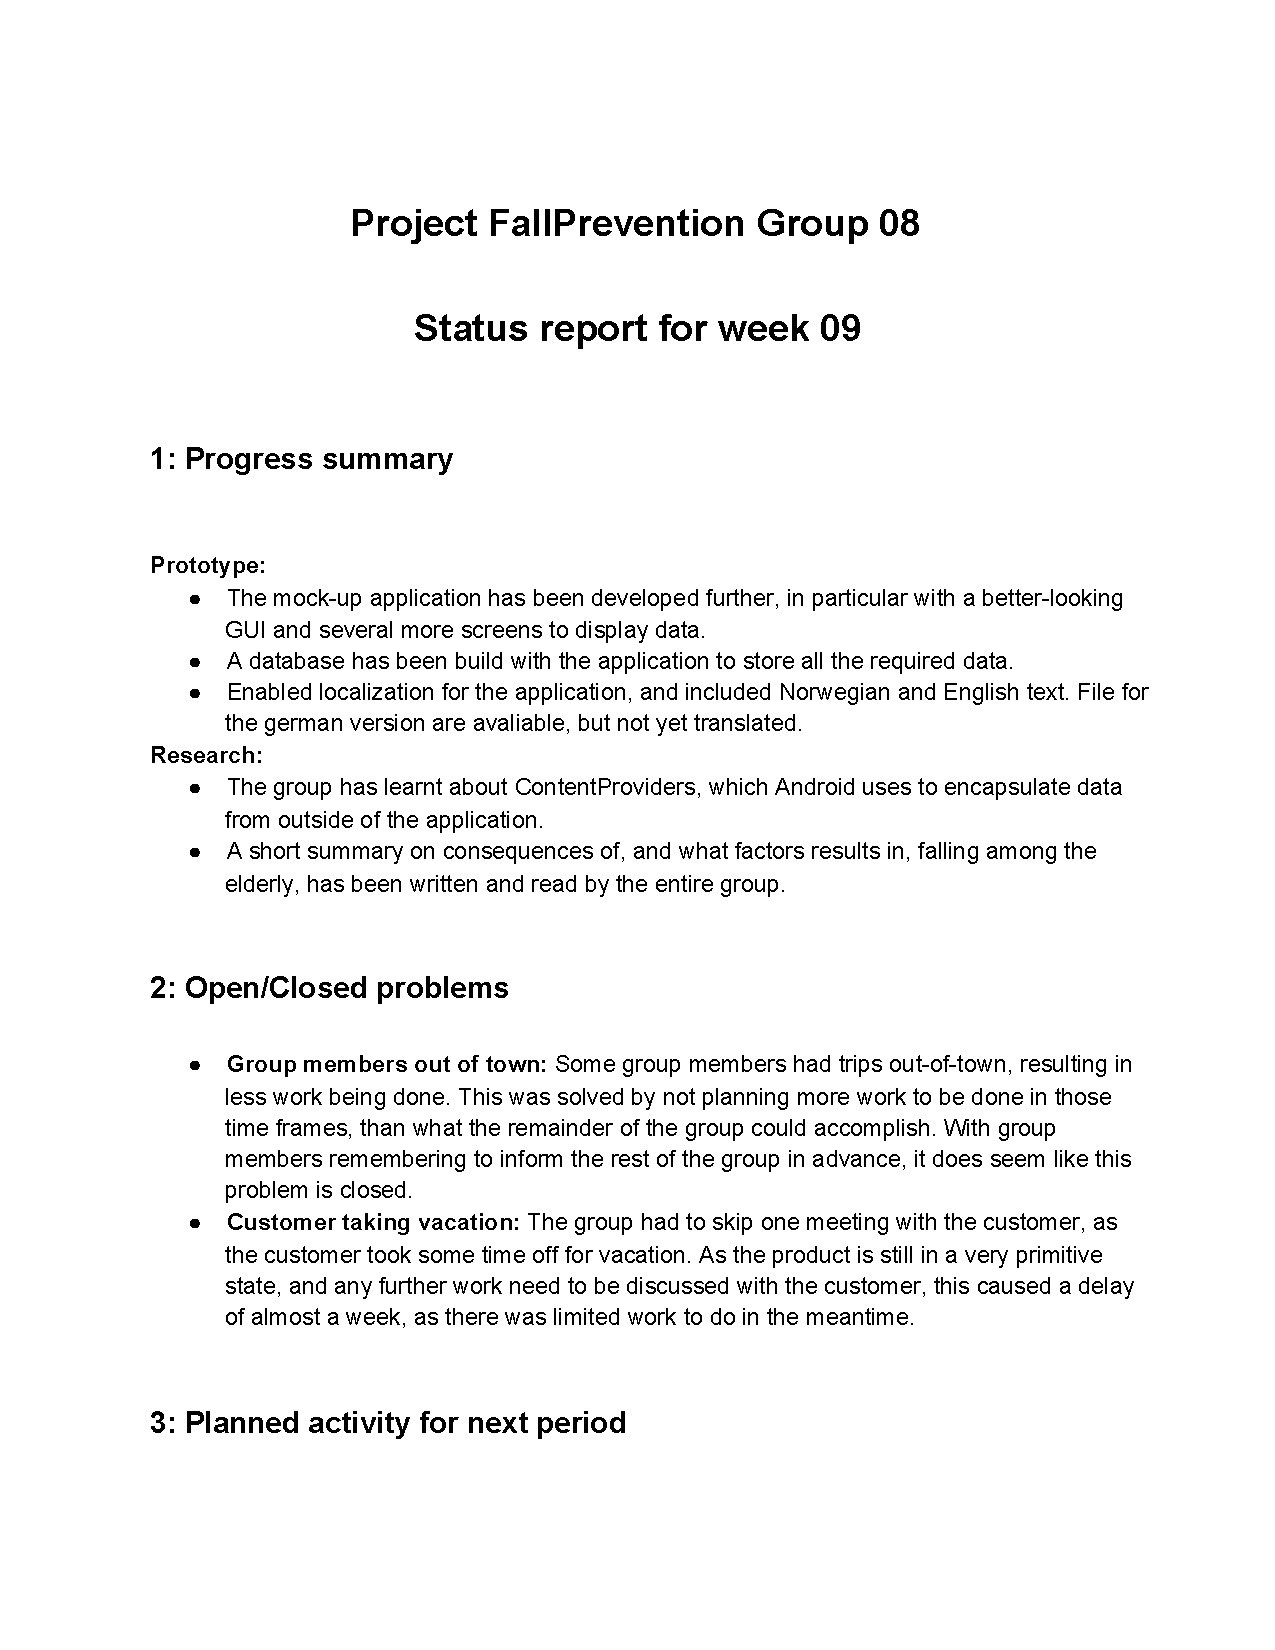
\includepdf[pages={-}]{Res/StatusReportWeek9}

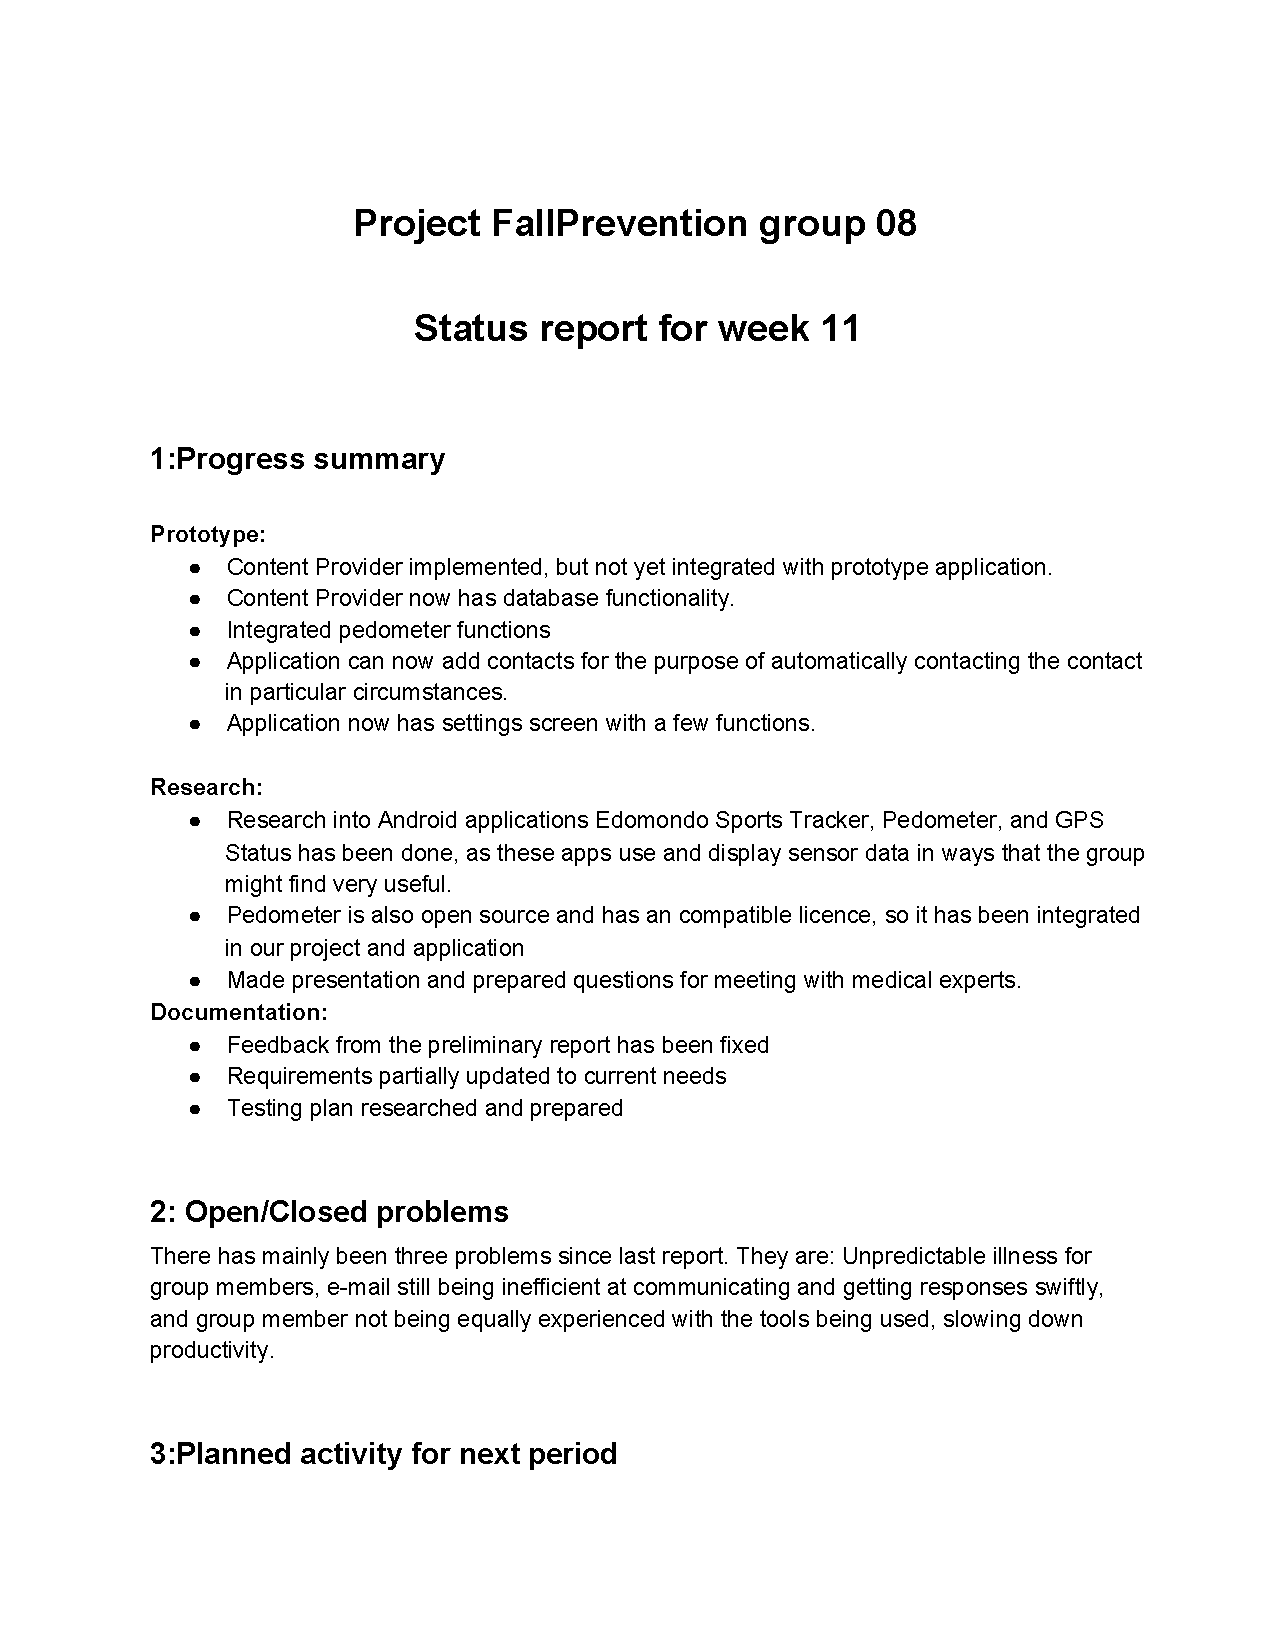
\includepdf[pages={-}]{Res/StatusReportWeek11}

\chapter{Test results}
Here is a copy of feedback the group received from the customer when the application was deployed for testing. 
\label{appendix:testResults}
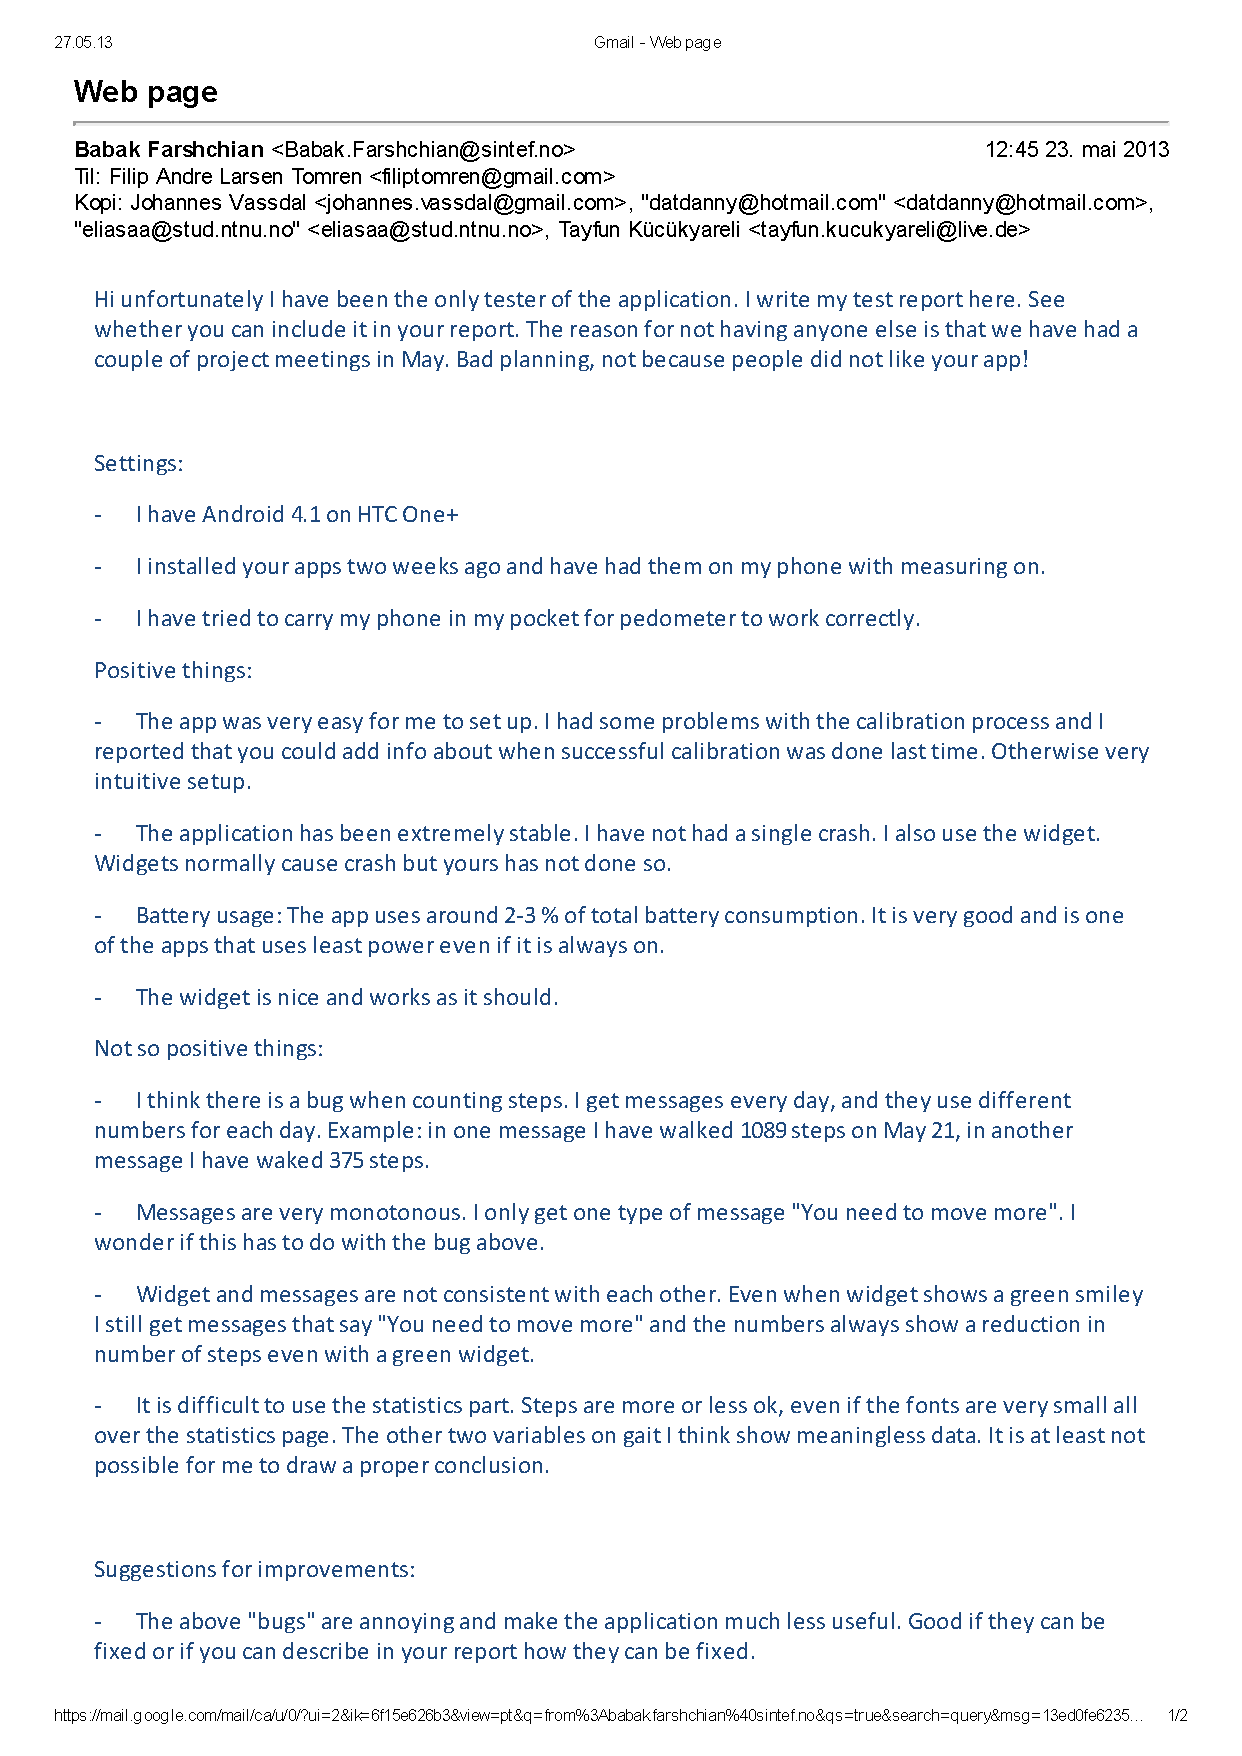
\includepdf[pages={-}]{Res/TestingSummaryBabak}
\subsection{Summary of interview with medical professionals}
This is a summary of the information gathered by a meeting with two medical professionals and the customer.
\textbf{Present:} All group members, Babak Farshchian, Jorunn L. Helbostad, Beatrice Vereijken \\
\textbf{Time:} 14.15-15.37\\
\textbf{Place:} St.Olavs Hospital\\
The plan was to have a short presentation, a short GUI demonstration, and then discuss and interview with the interviewees. \\
\subsubsection*{Feedback on Interface and Presentation of the program}
\begin{itemize}
\item Immediate and summarized feedback was desired, as it would be more helpful than feedback later.
\item A focus on falling is not a selling point, try health or lifestyle instead
\item Menu is not obvious to people without android experience
\item Interface seems too complex for target groups
\item Text might be too small
\item Graph needs more contrast 

\end{itemize}

\textbf{Feedback on program functionality}
\begin{itemize}
\item Feedback should be tailored to particular groups
\item Self-testing can be useful for reducing risk and keeping awareness,
\item Small tests to measure reaction time, for example reaction to light or sound
\item Researchers could also be interested in data gathering
\item Measuring transitions between sitting/lying and standing up
\item Compare behavior on a weekly basis will give an overview of whether things are good or not
\end{itemize}

\textbf{Feedback on medicinal stuff}
\begin{itemize}
\item Preventing inactivity over time is useful to reduce risk
\item People with stability problems increase risk when moving much
\item Variable gait pattern is useful for predicting risk
\item Step time is more robust (and hopefully easy to measure)
\item A common exercise is to take a step forwards, sideways, backwards, sideways (measuring a box)
\item People in risk group are those who cut out walking, taking the bus, want help from others around the house
\item Irregularity in speed and length is important to look for
\item Appropriate movement amount for gender and age group is usually known
\item Time needed to turn in place
\end{itemize}

\chapter{Time-sheet}
Here is the time-sheet used to log time spent working on the project.
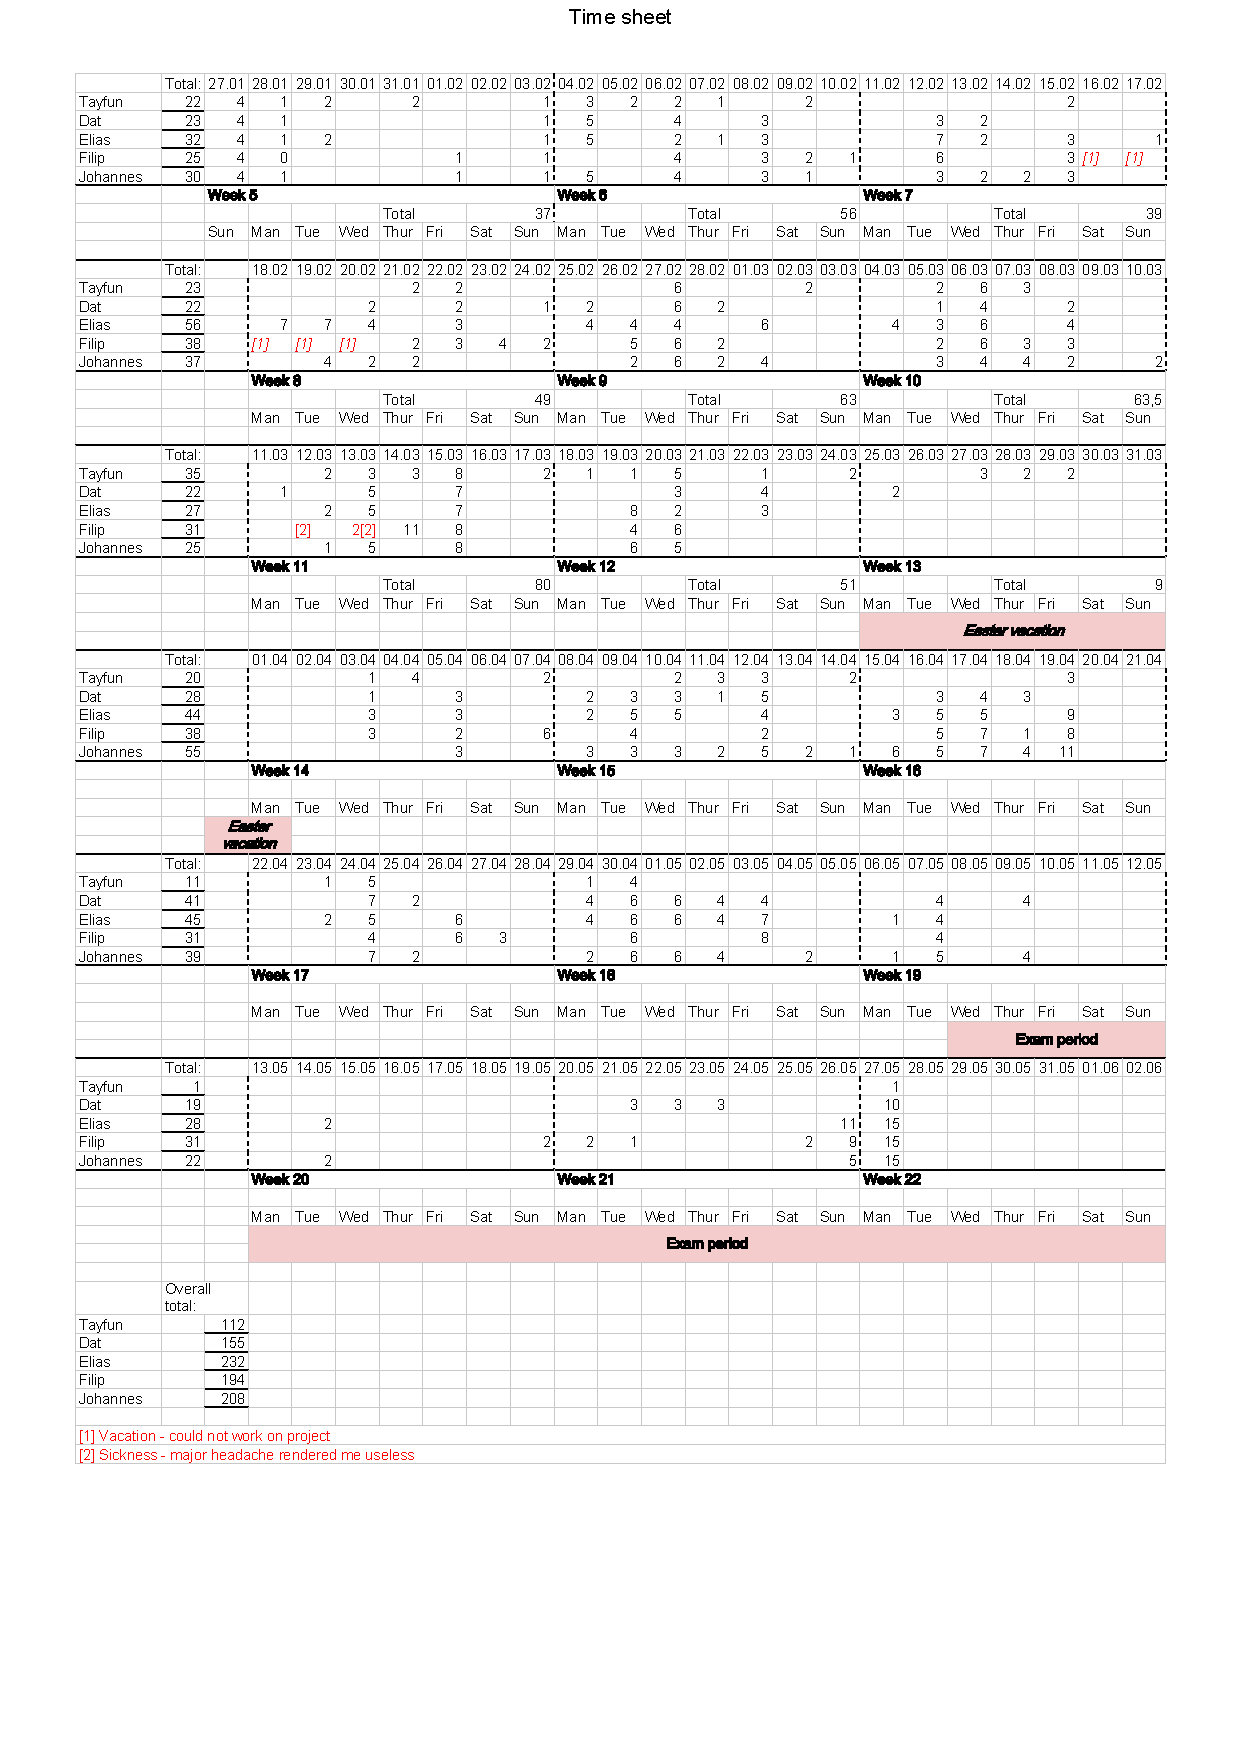
\includepdf[pages={1}]{Res/TimeSheet}
\chapter{User Stories}
\label{ref:userStories}
\section{Scenario 1: Ole Pedersen has osteoporosis}

\subsection*{Scenario 1a}
Ole Pedersen has osteoporosis, and has therefore been ordered by his doctor to use the program to help identify the risks involved with his everyday movements. He has been given an android phone by the hospital, and has been ordered to wear the phone in his pocket for a few days. Even though Ole Pedersen normally leaves his phone on the bedstand, he remembers to bring it with him almost every day, because the doctor said it was only temporary.
	At the next consultation, the doctor discusses the data provided by the phone.
	
	\subsection*{Scenario 1b}

Dr. Rypdahl is responsible for the health of Ole Pedersen. She configures the program for Ole Pedersen, and issues him with a phone running the program. The program generates data that is sent to a central database, from which Dr. Rypdahl can read information on her local computer.

\subsection*{Scenario 1c}

Dr. Rypdahl studies the data generated by Ole Pedersen’s phone. The data shows several periods with high risk of falling. The data implies that Ole Pedersen was climbing. At their next consultation,  she therefore questions him about his activites during these periods of time, and he confesses that he climbed a chair to change the curtains.

\subsection*{Scenario 1d}

The data later shows that Ole Pedersen has a higher risk of falling than expected when walking to the store. Dr. Rypdahl decides to send Ole Pedersen to a physiotherapist in order investigate how he walks.

\subsection*{Scenario 1e}

Ole Pedersen has been assigned to the physiotherapist Hanne Falk. Before their first consultation, she studies the data generated by the program. The data indicates that Ole Pedersen walks with a limp in his right foot, so she knows where to look first during the consultation.

\subsection*{Scenario 1f}

Hanne Falk asks Ole Pedersen to wear the phone for a few days between every consultation, so that she can monitor his progress improvement, and see whether there are any side effects of the treatment. By studying the data for a while before every consultation, she knows what areas to focus her treatment on.

\section{Scenario 2: A worried relative}


\subsection*{Scenario 2a}

Odd Einar has a relative he is worried about, as his grandmother, Caroline, is growing old and frail. Therefore he gives her an android phone with the program installed, and asks her to carry it around with her. He then check the program regularly, looking for problematic patterns in her movement. He can then tell her doctor that she needs some help in avoiding that behaviour in the future.

\subsection*{Scenario 2b}
Odd Einar feels that the doctor is too slow in being helpful, so he makes the phone send him a warning if the risk increases past a certain threshold. This warning contains information about what his grandmother is doing, and a few suggestions about what can be done to avoid this. He then goes out and helps her redecorate, so she wont have to do the risky behaviour as often. 

\subsection*{Scenario 2c}
Caroline has an accident, and falls in the living room and breaks something important. She is unable to get help, but she was wearing the phone at the time. Then the phone registers that something is wrong, and sends an message to Odd Einar. 

\subsection*{Scenario 2d}

Following the accident, Caroline is hospitalized. Fortunately, she recovers completely, but Odd Einar is worried that it might happen again. He therefore asks the doctor to examine the data in the time leading up to the accident. The doctor finds that the grandmother’s walking was less stable the last minutes before the accident. Even though the doctor does not understand why this happened, Odd Einar configures the program so that it triggers an alarm when it detects a similar pattern. When the alarm is sounded, Caroline knows that she should sit down and relax for a while.


\section{Scenario 3: A troublesome user}

\subsection*{Scenario 3a}

Elise has received an Android phone and has been told by the Doctor to carry it around at all times. Given the command she always puts the phone in her purse when she is going outside. Because the phone need to be in the pocket for the program to work properly, the data generated does not correspond to reality, as the program thinks she is doing something completely different from what she really does. Eventually the program discovers that Elise is using it in the wrong way, and a warning message pops up on the phone that tells her to put the phone in her pocket.

\subsection*{Scenario 3b}

Elise likes to keep in touch with her friends and relatives, and because the new phone provided by the hospital can be taken with her anywhere she goes, she uses it to send SMS messages and call her friends. When she holds the phone in her hand, it generates movement data that is not based on hip movement, so it is just noise for the Doctor who is reading her data use. 
The program handles this noise in two ways: It stops transmitting data while the screen lock is turned off. Also, it ignores large, sudden movements, such as the removal of the phone from the pocket.

\section{Scenario 4: The gamer}

\subsection*{Scenario: 4a}

Timmy likes to play video games and rarely goes outside. His mother notices that he tends to waddle a lot when he is home and is worried. She instructs him to use the program for a week so she can determine if he has any problem walking around outside.

\subsection*{Scenario: 4b}

Timmy has been walking around with the program monitoring his movements for a week, while his mother has regularly received reports about his risk of falling. As the system fails to detect any anomalies in Timmy’s motion pattern, his mother need not to worry about his way of walking.

\section{Scenario 5: The scoundrel}

\subsection*{Scenario 5a}

Jonas Jensen makes a living from stealing old people’s valuables. He learns about the program from one of his “colleagues” that steals medicine from the local hospital. Jonas immediately realizes that if he gains access to the database, he can learn which people are unable to defend themselves against a robber, or use the data to learn when the owner is walking outdoors, so that the house is alone and can be robbed safely. 





\section{Scenario 6: The boy with narcolepsy}

\subsection*{Scenario 6a} 
Alain Basel is a 6 years old boy. Before three years Dr. M.Stone has detected genetic narcolepsy on him. Since that date both Dr. M. Stone and the Family Basel are trying to help Alain with his problem. The Doctor tries to figure out how often Alain has his falling downs/knock outs. But for the reason that this analyse can only be once a week Dr. M. Stone need a method for detecting Alain every time. Something like an mobile gadget on Alain’s body could be the solution. For the problem that Alain does not like medical gadgets, in that way that he throws them away, a mobile phone could gain acceptance from Alain.




\section{Scenario 7: Mrs. Mc Hipo with the new artificial hip and the new product need to been tested}

Mrs Mc Hipo got a new artificial hip with a new technology. The doctors from the hospital are not sure if the new material with more polyethyl could help to walk easier without any walk diffiulties. For the reason that the doctors want to detect how good the new product is they give Mrs Mc Hipo a smart phone for detecting the products quality.
\end{appendices}